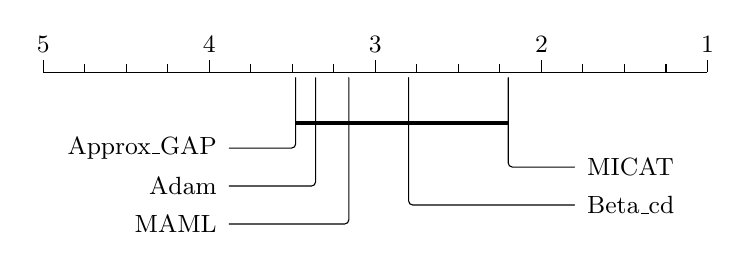
\begin{tikzpicture}[
  treatment line/.style={rounded corners=1.5pt, line cap=round, shorten >=1pt},
  treatment label/.style={font=\small},
  group line/.style={ultra thick},
]

\begin{axis}[
  clip={false},
  axis x line={center},
  axis y line={none},
  axis line style={-},
  xmin={1},
  ymax={0},
  scale only axis={true},
  width={\axisdefaultwidth},
  ticklabel style={anchor=south, yshift=1.3*\pgfkeysvalueof{/pgfplots/major tick length}, font=\small},
  every tick/.style={draw=black},
  major tick style={yshift=.5*\pgfkeysvalueof{/pgfplots/major tick length}},
  minor tick style={yshift=.5*\pgfkeysvalueof{/pgfplots/minor tick length}},
  title style={yshift=\baselineskip},
  xmax={5},
  ymin={-3.5},
  height={4\baselineskip},
  xtick={1,2,3,4,5},
  minor x tick num={3},
  x dir={reverse},
  title={},
]

\draw[treatment line] ([yshift=-2pt] axis cs:2.2, 0) |- (axis cs:1.7833333333333334, -2.5)
  node[treatment label, anchor=west] {MICAT};
\draw[treatment line] ([yshift=-2pt] axis cs:2.8, 0) |- (axis cs:1.7833333333333334, -3.5)
  node[treatment label, anchor=west] {Beta\_cd};
\draw[treatment line] ([yshift=-2pt] axis cs:3.16, 0) |- (axis cs:3.8966666666666665, -4.0)
  node[treatment label, anchor=east] {MAML};
\draw[treatment line] ([yshift=-2pt] axis cs:3.36, 0) |- (axis cs:3.8966666666666665, -3.0)
  node[treatment label, anchor=east] {Adam};
\draw[treatment line] ([yshift=-2pt] axis cs:3.48, 0) |- (axis cs:3.8966666666666665, -2.0)
  node[treatment label, anchor=east] {Approx\_GAP};
\draw[group line] (axis cs:2.2, -1.3333333333333333) -- (axis cs:3.48, -1.3333333333333333);

\end{axis}
\end{tikzpicture}